\documentclass[12pt,a4paper]{book}
\usepackage[utf8]{inputenc}
\usepackage[T1]{fontenc}
\usepackage[main=english,spanish,es-tabla]{babel}

% \usepackage{hyphenat}
% \hyphenation{apren-di-zaje pro-fun-do}

\usepackage[left=2.5cm,right=2cm,top=2cm,bottom=1.7cm,includefoot,includehead,headheight=16pt]{geometry}

\usepackage{lipsum}

% Bibliografía
% \usepackage[style=authoryear]{biblatex}
% \addbibresource{bibliografia.bib}
\usepackage[authoryear,round]{natbib}
\bibliographystyle{unsrtnat}

% Control sobre los márgenes
\setlength{\topmargin}{-1cm}
\setlength{\textheight}{24cm}
\setlength{\linewidth}{3cm}

% Estilo
\usepackage{amsmath,amssymb,amsfonts,stackrel,hyperref}
% \numberwithin{equation}{section}
\usepackage{graphicx,color}
\definecolor{verde}{RGB}{0, 83, 62}
\usepackage{setspace}
\renewcommand{\baselinestretch}{1.2}


% Tablas
\usepackage{tabularx,multirow,rotating,longtable}

% Código
\usepackage{listings} 
\usepackage[mathscr]{euscript}
\lstdefinestyle{estiloMUICD}{
    backgroundcolor=\color{black!5!white},
    commentstyle=\color{green!60!black},
    keywordstyle=\color{blue},
    numberstyle=\footnotesize,
    stringstyle=\color{black!40!white}\ttfamily,
    basicstyle=\small\ttfamily,
    breakatwhitespace=false,
    breaklines=true,
    captionpos=b,
    keepspaces=true,
    numbers=left,
    numbersep=8pt,
    showspaces=false,
    showstringspaces=false,
    showtabs=false,
    tabsize=2
}
\lstset{style=estiloMUICD}


% Tikz
\usepackage{tikz}
\usetikzlibrary{arrows}

% Encabezados
\usepackage{fancyhdr}
\fancyhf{}
\fancyhead{}
\pagestyle{fancy}
\fancyhead[LE,RO]{\thepage}
\fancyhead[LO, RE]{\leftmark}
\renewcommand{\chaptermark}[1]{\markboth{#1}{}}
\renewcommand{\sectionmark}[1]{\markright{#1}}
\pagestyle{empty}

% Glosarios y nomenclaturas
\usepackage[toc,nonumberlist]{glossaries}
\makeglossaries

% Introduzca de cada término del glosario su nombre y su descripción
\newglossaryentry{subject}{
    name={Subject},
    description={An individual runner included in the dataset. Each subject may contribute one or more running sessions.}
}

\newglossaryentry{session}{
    name={Session},
    description={A continuous treadmill run (approximately 60 seconds) recorded from a single subject. Each session yields multiple gait cycles.}
}

\newglossaryentry{cycle}{
    name={Cycle},
    description={A gait cycle defined as the interval between two successive foot touchdowns of the same foot, including both stance and swing phases.}
}


\newglossaryentry{mocapsys}{
    name={MoCap system},
    description={Motion Capture System. A system that uses multiple cameras and reflective markers to record the three-dimensional positions of anatomical landmarks on a subject during movement, enabling precise measurement and analysis of body kinematics.}
}


\begin{document}
% \glsaddall
\frontmatter
\begin{titlepage}
\centering
	
\includegraphics[height=4cm]{ images/logo_informatica_s.png}\\
	\vspace{0.25cm}
 	{\Large \textsc{{Universidad Nacional\\ de Educación a Distancia}}}\\
 	\vspace{0.8cm}
	{\Large Escuela Técnica Superior de Ingeniería Informática}\\
	\vspace{0.25cm}
	\vspace{1.5cm}
    \begin{spacing}{2}
  	{\textsc{\Huge Injury detection in runners using anthropometric and 3D marker-based kinematic data.}}
    \end{spacing}
	\vfill
	{\Large Adrián José Zapater Reig}\\
	\vspace{0.3cm}
	\begin{tabular}{ll}

	\large Supervisor: & \large Olga C. Santos Martín\\
	% \vspace{0.3cm}\\
	\large Co-supervisor: & \large Miguel Ángel Portaz Collado\\
        \large Co-supervisor: & \large Dr. Javier Gámez Payá 
	\end{tabular}
	
	\vfill
	{\Large Master's Thesis}\\
	\vspace{0.3cm}
	{\large Máster Universitario\\ en Ingeniería y Ciencia del Dato}\\
	\vspace{0.25cm}
	Septiembre 2025
\end{titlepage}
\cleardoublepage{}

\begin{flushright}
\section*{Agradecimientos}
[Quisiera dedicar \ldots]
\par\end{flushright}    



\cleardoublepage{}
\include{otros/summary}

\cleardoublepage{}
\selectlanguage{english}%
\noindent \begin{center}
\section*{Abstract}
\par\end{center}

\lipsum[1-2]

\vspace{0.5cm}
\begin{flushleft}
\textbf{Keywords}: keyword1, keyword2, keyword3
\end{flushleft}
\selectlanguage{spanish}%

%\newpage
\printglossary


\tableofcontents
\listoffigures
\renewcommand{\listtablename}{List of Tables}
\listoftables


%\newpage
\mainmatter
\pagestyle{fancy}

\chapter{Introduction}\label{chap:introduction}
%Motion analysis is the systematic study of human movement, and it is a key component of many fields, including biomecanics, medicine and sports science.
%Kinematics is the study of the motion of objects without considering the forces causing the motion.
-- To populate after objectives.

Can we detect running injuries using kinematic data? -> Lots of research exists that relates injuries to training load, physiological factors that require logitudinal data to be collected during a long period of time

Lots of research into injury risk prediction, but not much into injury detection.
% Research in the domain of ML for injury risk prediction in sports has grown steadily over the last 10 years (https://bjsm.bmj.com/content/59/7/491)


Proof that MAchine learning has been used successfully in the field of biomechanics 




\section{Motivation}\label{sec:intro-motivation}
-- Why? Why are we here?
-- Narrative of the problem
-- Real-world problem (running injuries), impact/costs, current practical gap.
-- My personal interest in the topic?
-- Lack of conclusive research, lack of variety of techniques, etc...

\section{Context and Collaboration}\label{sec:intro-context}
-- Collaboration with Javier, ...
-- Source paper: what it proposes, what you adopt, what you don't.
    -- The value that the paper brings to the community amnd why it is important + effect on community.
    -- What could be improved?
    -- Limitations, assumptions, etc..

\section{Problem Statement \& Hypotheses}\label{sec:intro-problem-hypotheses}
-- Clear and verifiable
-- Detection of running injury from kinematic data. (Rephrase better)


\section{Objectives an Scope}\label{sec:intro-objectives-scope}
% -- concise, measurable, and testable
% -- Scope, limits, and assumptions
% -- What does the source study not cover? What is out of scope for us?
%     - Longitudinal analysis
%     - Follow-up on subjects to track evolution of the injury.
%     - Temporal information about the injury (chronic, not chronic, recent, coping, etc...)
Objectives:
O1: The primary objective is to evaluate how well do 4 classical ML models trained on the biomechanical variables provided in the running-injury dataset (N=1402 runners) detect injury status, and determine whether any achieves AUC-ROC > 0.7.

O2: Assess whether advanced deep learning models (Unilateral LSTM, Bilateral LSTM, MC-DCNN) trained on time-series kinematic data significantly (p \le 0.05) outperforms the best baseline by \(\delta\) > 0.05 on the primary metric (AUC-ROC) with 95\% Confidence Interval over 5-fold cross-validation.

O3: Apply post-hoc interpretability techniques (SHAP and saliency maps) to interpret black-box models and identify key kinematic features that contribute most to injury detection.












- to develop a model that can detect running injuries from kinematic data.
- to build on top of the work done by the source paper.
- To use Machine Learning to solve 


Hypothesis:
- Can we detect running injuries using kinematic data (without force data) without longitudinal data?
- We learn from AI system to 

\section{Contributions}\label{sec:intro-contributions}
-- What is the value of the research?
-- What assets do I leave behind?
-- Methods, data, code, results, ....

\section{Document Structure}\label{sec:intro-structure}
-- Overview of the document structure, chapters, sections, etc...

\chapter{Estado del Arte}


\chapter{Materials and Methods}\label{chap:materials-methods}
This chapter introduces the materials and datasets provided in the source paper \citep{Ferber2024}. We then describe how the data were preprocessed and explored, explain how the models were implemented, trained, and evaluated, and finally present the methods used to analyse model explainability.

\section{Data and Materials}\label{sec:method-data-materials}
As part of \citet{Ferber2024}, the authors have published a dataset of 1798 \glspl{subject} running or walking on a treadmill captured using multi-camera 3D \gls{mocapsys}. The dataset is composed of raw 3D marker data of each \gls{session}, descriptive biomechanical variables derived from the marker data for each session and demographic and anthropometric metadata of the subjects. Additionally, the matlab code for the preprocessing of the data, the calculation of the kinematic variables and tutorial notebooks that help lustrate how to use their library and read the data from the folder structure are also provided. Although both walking and running data is provided, we have used exclusively running data. From this point onwards, walking data is ignored for brevity.

\subsection{Measurement protocol}\label{subsec:measurement-protocol}
The complete measurement protocol is described in \citet{Ferber2024}. In this subsection, we provide a summary of the aspects that are most relevant for the methods and analyses presented in this thesis.

The raw marker data was collected using high-speed optoelectronic infrared-based motion capture cameras (MX3/Bonita, Vicon, Oxford, UK) were used to record the position of 9 mm spherical retro-reflective markers attached to anatomical landmarks of the subjects at either 120 Hz or 200 Hz. Depending on the lab, eight or three cameras were used. Below we list and describe the three sets of markers that were used.
\begin{itemize}
    \item \textbf{Core}: Markers attached to the following anatomical landmarks: medial and lateral malleoli, medial and lateral femoral condyles, and greater trochanters.
    \item \textbf{Additional}: Markers attached to the following anatomical landmarks: bilateral 1st and 5th metatarsal heads, distal aspect of the shoe, tibial tuberosity, anterior superior iliac spines, and iliac crests;
    \item \textbf{Clusters}: 3 or 4 markers placed on rigid shells attached to the following anatomical landmarks: sacrum, bilateral thigh and shank, and posterior aspect of both shoes.
\end{itemize}

During the recording of the sessions of all 1798 subjects the 'core' and 'cluster' set of markers were used. The additional set was only used during the recording of the sessions of 1082 subjects. Figure \ref{fig:marker_position} shows the lower body of a subject and the three sets of markers.

\begin{figure}[ht]
    \begin{centering}
    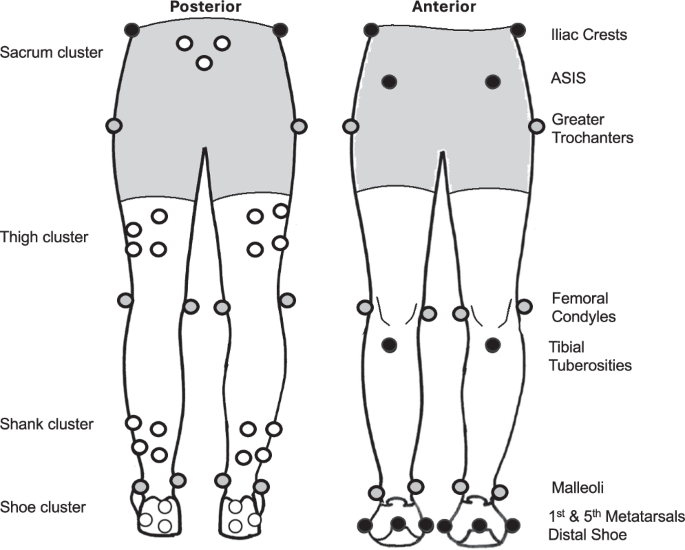
\includegraphics[width=0.5\columnwidth]{images/billateral_marker_position.png}
    \par\end{centering}
    \caption{Position of markers on the subjects. Grey markers correspond to core set of markers set, black to additional set and white to the clusters set.}
    \label{fig:marker_position}
\end{figure}

% TODO: Explain the recording procedure: Warm up, duration, discard, etc...

\subsection{Dataset Description}\label{subsec:method-dataset-description}
As described above, the dataset contains two complementary components: (i) session-level metadata stored as tabular files, and (ii) motion-capture marker data together with derived kinematic variables per session. Below we describe each component and list the variables that are available for analysis.

\paragraph{Metadata File (tabular) The metadata file is provided as a CSV file: \texttt{run\_data\_meta.csv}. Each row corresponds to a single treadmill session recorded for a subject. It contains anthropometric and demographic variables.
\begin{itemize}
    \item \texttt{sub\_id}: Unique subject identifier.
    \item \texttt{datestring}: Session recording date.
    \item \texttt{filename}: Session filename used to locate the marker json file for the session.
    \item \texttt{speed\_r}: Treadmill belt speed (m/s).
    \item \texttt{age}: Subject's age (years).
    \item \texttt{Height}: Body height (cm).
    \item \texttt{Weight}: Body weight (kg).
    \item \texttt{Gender}: Subject gender.
    \item \texttt{DominantLeg}: Dominant leg (Left/Right/Ambidextrous).
    \item \texttt{InjDefn}: Injury severity reported by the subject choosing between 4 options: (1) No Injury, (2) Continuing to train in pain, (3) Training volume/intensity affected, (4) Minimum of two workouts missed in a row.
    \item \texttt{InjJoint}, \texttt{InjSide}, \texttt{SpecInjury}, \texttt{InjDuration}: Primary injured joint, side (Left/Right), Specific injury diagnosis from medical professional, and for how long has the subject had the injury.
    \item \texttt{InjJoint2}, \texttt{InjSide2}, \texttt{SpecInjury2}: Secondary injury information (if applicable).
    \item \texttt{Activities}: Subject reported athletic activities performed on a regular basis.
    \item \texttt{Level}: Self-reported level of athletic activity (recreational/competitive).
    \item \texttt{YrsRunning}: Number of years subject has been running on a regular basis.
    \item \texttt{RaceDistance}: Preferred race distance.
    \item \texttt{RaceTimeHrs}, \texttt{RaceTimeMins}, \texttt{RaceTimeSecs}: Preferred race distance best time.
    \item \texttt{YrPR}: Year of preferred race distance personal best time.
    \item \texttt{NumRaces}: Number of races completed per year.
\end{itemize}

\paragraph{Marker and descriptive biomechanical data (Hierarchical)} For each session, 3D positions of reflective markers and descriptive variables derived from those markers are provided.
\begin{itemize}
    \item \textbf{Recording frequency} Frequency of the recording in Hertz (Hz). Either 120 Hz or 200 Hz depending on the lab.
    \item \textbf{Joint Marker Neutral}: 3D coordinates of the individual markers of the core and additional marker sets while the subject is standing in neutral position.
    \item \textbf{Cluster Marker Neutral}: 3D coordinates of the individual markers in the cluster marker set while the subject is standing in neutral position.
    \item \textbf{Dynamic Marker data}: 3D coordinates at each of the frames of the recording for the individual markers in the cluster marker set.
    \item \textbf{Descriptive biomechanical variables}: Set of 77 variables derived from the 3D coordinates Marker data. Calculated for Left and Right side of the body.
\end{itemize}

It must be noted that \texttt{Joints} and \texttt{Neutral} coordinates do not represent the true anatomical centres, only the centres of the markers on the skin of the subject.
Only 33 of the 77 descriptive biomechanical variables are populated per side, the rest all contain 0 for all values of all sessions, this totals 66 populated descriptive variables in total. Table \ref{tab:met-desc-variable-init} describes the variable set per side.

\begin{table}[ht]
    \centering
    \caption[Populated Descriptive Variables Summary]{Summary of the Descriptive Biomechanical Variables that are populated\label{tab:met-desc-variable-init}}
    \begin{tabular}{lp{0.6\textwidth}}
    \hline
    Variable & Category \\
    \hline
    Step width (m) & Temporal-spatial \\
    Stride rate (steps/min) & Temporal-spatial \\
    Stride length (m) & Temporal-spatial \\
    Swing time & Temporal-spatial \\
    Stance time & Temporal-spatial \\
    Peak drop angle & Pelvis kinematics \\
    Drop excursion & Pelvis kinematics \\
    Dorsiflexion peak angle & Ankle kinematics \\
    Ankle Eversion peak angle & Ankle kinematics \\
    Ankle Rotation peak angle & Ankle kinematics \\
    Ankle Eversion excursion & Ankle kinematics \\
    Ankle Rotation excursion & Ankle kinematics \\
    Ankle Eversion \% of stance & Ankle kinematics \\
    Knee Flexion peak angle & Knee kinematics \\
    Knee Adduction/abduction peak angle & Knee kinematics \\
    Knee Rotation peak angle & Knee kinematics \\
    Knee Adduction/abduction excursion & Knee kinematics \\
    Knee Rotation excursion & Knee kinematics \\
    Hip Extension peak angle & Hip kinematics \\
    Hip Adduction peak angle & Hip kinematics \\
    Hip Rotation peak angle & Hip kinematics \\
    Hip Adduction excursion & Hip kinematics \\
    Hip Rotation excursion & Hip kinematics \\
    Foot progression angle & Foot kinematics \\
    Heel-strike angle & Foot kinematics \\
    Medial heel whip excursion from toe-off & Foot kinematics \\
    Ankle eversion peak velocity & Joint velocities \\
    Ankle rotation peak velocity & Joint velocities \\
    Knee adduction peak velocity & Joint velocities \\
    Knee abduction peak velocity & Joint velocities \\
    Hip abduction peak velocity & Joint velocities \\
    Knee rotation peak velocity & Joint velocities \\
    Hip rotation peak velocity & Joint velocities \\
    Pelvic drop peak velocity & Joint velocities \\
    Pronation onset \% of gait cycle & Foot timing \\
    Pronation offset \% of gait cycle & Foot timing \\
    Vertical oscillation (mm) & Vertical oscillation \\
    \hline
    \end{tabular}
\end{table}

All descriptive variables follow the interpretations described in \citet{Bartlett2014}. Unless specified explicitly in the table, the units are degrees for angles and excursions, and degrees/s for joint velocities. Excursions are also commonly known as range of motion (ROM) in the literature. 
% TODO: Explain important biomechanical concepts like dorsiflexion, eversion, etc...


\subsection{Code Description}\label{subsec:method-code-description}
Python was the main language used in this project, although several scripts were implemented in \GLS{matlab} for the data acquisition and extraction stages. Matlab was also used to preprocess the dataset, following the procedure described in the source paper. All code created for this project and used to generate the reported results has been made publicly available for reproducibility \cite{Zapater_Reig_Running_Injury_Clinic_2025}.  

The MATLAB reference implementation published with the dataset in \citet{Ferber2024} was employed as part of this work. The corresponding MATLAB scripts have been included in the repository under the \texttt{supplemental\_material} folder for consultation.  

The following assets are the most relevant components of the repository:  

\paragraph{Notebooks}  
Jupyter notebooks used during development. These capture the iterative process across the different phases of the project and the reporting of results.

\paragraph{\texttt{core} Package}  
Python package containing the core functionality used in the notebooks. It includes classes, functions, and constants to orchestrate data extraction, preprocessing, feature engineering, model training, and evaluation.  

\paragraph{\texttt{gait\_kinematics.m}}  
Script provided with the source paper. It calculates joint angles and angular velocities from the \texttt{Dynamic Marker Data}, \texttt{Joint Marker Neutral}, and \texttt{Cluster Marker Neutral} files. Anatomical segment coordinate systems are constructed from the neutral marker data, segment motion is tracked using the dynamic marker data, and XYZ Cardan joint angles and angular velocities are computed. The script returns:  
\begin{itemize}
    \item \texttt{Angles}: per-frame joint/segment angles for the left/right ankle, knee, hip, as well as foot and pelvis segments (degrees).
    \item \texttt{Velocities}: per-frame angular velocities for the same structures (deg/s).
    \item \texttt{jc}: estimated joint centre positions (pelvis, hips, knees, ankles).
\end{itemize}

\paragraph{\texttt{gait\_steps.m}}  
Script also provided with the source paper. It calculates descriptive biomechanical variables from the \texttt{Dynamic Marker Data}, \texttt{Cluster Marker Neutral}, \texttt{Angles}, and \texttt{Velocities}. The script returns:  
\begin{itemize}
    \item \texttt{event}: gait cycle events by side (touchdown, mid-stance, toe-off, heel whip).
    \item \texttt{Descriptive biomechanical variables}: as defined in Table~\ref{tab:met-desc-variable-init}.
\end{itemize}

\paragraph{\texttt{processing\_source\_data.m}}  
Script implemented for this project to process the metadata file and marker-data JSON files. Joint angles and angular velocities are computed by calling \texttt{gait\_kinematics.m} and \texttt{gait\_steps.m}. The outputs are converted into tabular format for the exploratory data analysis (EDA) stage. Sessions without valid running data, or those where MATLAB preprocessing failed, were excluded.

\subsection{Data Extraction}\label{subsec:data-extraction}
% -- How Kinematic variables are derived.
% -- How we obtained angles, angular velocities from matlab and events...
% -- Internal processing assumptions
% -- Axis reconstruction
% -- Estimations
% -- Focus on the Stance because computed variables are also focused there. Same reference paper. Or alternatively put in state of the art and justify here that we think it is better this way.
% TODO: How to integrate EDA and Preprocessing, since it is related...

... Using 





% TARGET: End with a summary of the tabular and time-series data that we have extracted



\section{Exploratory Data Analysis (EDA)}\label{sec:method-eda}
% -- Exploration → Extraction → Preparation, with concrete checks and figures:
% -- Tabular data Exploration (sanity and distributions)
% -- Dataset inventory (sessions per runner, class prevalence per runner, cycles/session).
% -- Missing-ness map (metadata \& signals); strategy preview (drop/impute).
% -- Outliers: per-joint angle/velocity ranges, z-score >3 heat-map by runner (flag sensors/markers).
% -- Dimensionality previews: PCA/t-SNE to see separability.


% -- Time-series data Exploration:
% -- Visuals: overlay of 20 random stance cycles per class; Markers, Angles, Velocities, ...
% -- Analysis of curves
% -- Extraction (curve-level descriptors)


% -- Preparation (decisions fixed before modelling)

% -- Group-aware split policy (runner-level), ensuring no cycle leakage across folds.
% -- Class-imbalance diagnostics (AUC-PR baseline, per-runner prevalence plots).
% -- Filtering rules for cycles/sessions (min cycles per session, quality thresholds).

% -- Final feature set(s) to carry forward (e.g., summaries, PC scores, raw curves for DL)

% TODO: Maybe we keep outliers and filering here?
Steps:
- 


\section{Pre-processing}\label{sec:method-preprocessing}
-- Tabular:
    -- filtering, subject identification, outliers, cleaning, etc..
    -- Final dataset creation -> Give name to track

-- Time-series:
    -- Extraction of angles and angular velocities as mentioned in literature.
    -- Extraction of events
    -- Combination of events and TS
    -- Cycle Segmentation and normalization -> Reference papers either here or in SOTA.

\subsection{Feature Engineering}\label{subsec:method-feature-engineering}
-- Transformations and feature extraction
    -- Dominant Leg -> VIF reduction
    -- Obtaining a representative curve
        -- Curve registration attempt and Actual result

-- Feature selection:
    -- MRMR for feature selection

\subsection{Feature Selection}\label{subsec:method-feature-selection}
-- Transformations and feature extraction
    -- Dominant Leg -> VIF reduction
    -- Obtaining a representative curve
        -- Curve registration attempt and Actual result

-- Feature selection:
    -- MRMR for feature selection

% \subsection{Tabular Data}\label{subsec:method-tabular-data}
% -- Correlations mutual information, ...
% -- Collinearity: PCA, VIF, ...
% -- Left-right features - Dominant leg extraction
% -- Collinearity reduction

% \subsection{Timeseries Data}\label{subsec:method-timeseries-data}
% -- Segmentation: TD/TO, stance, swing, ...
% -- Normalisation/standardisation

\subsection{Final Feature Sets}\label{subsec:method-final-feature-sets}
-- Summary of the feature by dataset.

\section{Models}\label{sec:method-models}
\subsection{Baseline (Tabular)}\label{subsec:method-baselines}
\subsection{Deep Learning}\label{subsec:method-deep-learning}
-- Unilateral LSTM
-- Bilateral LSTM
-- Multimodal
-- TMAG
-- MC DCNN

-- Add special tuning for class imbalance, etc...
-- Architecture choices (hyperparameters, etc...)
-- class imbalance, oversampling, etc... TBD Where to put this? -> Explain in the models that used it. We will give results for each option individually.

\section{Evaluation Protocol}\label{sec:method-evaluation-protocol}
-- The blueprint before we run anything.
-- Questions/Hipothesis, grouping, leakage, validation scheme (group-aware train/val/test)
-- Evaluation protocol -> Measurements, statistics. How are we scoring the experimentriment. (Primary, Secondary metric, Threshold rule, ...).
-- Significance Tests. How do we know something is "Better" (DeLong's test)?
-- CI 95 \%
-- Research questions (RQs), validation scheme (group-aware train/val/test), splits, primary/secondary metrics.
-- Justify the choices , but do not present any results yet...

\subsection{Evaluation Metrics}\label{subsec:method-evaluation-metrics}
- AUC ROC + PR for class imbalance + Macro F1 score for threshold.

\subsection{Training and Validation Strategy}\label{subsec:method-training-validation-strategy}
-- Train, test, validation split.
-- Group-aware split policy (runner-level), ensuring no cycle leakage across folds.
-- Class-imbalance diagnostics (AUC-PR baseline, prevalence).

\subsection{Hyperparameter Tuning}\label{subsec:method-hyperparameter-tuning}
-- Grid search, random search, ...
-- Cross-validation, nested cross-validation, ...
-- Early stopping, ...
-- Hyperparameter tuning strategy.


\section{Explainability}\label{sec:method-explainability}
<Draft> This project would have been set up differently if the sole goal had been to build and deploy an injury detection model. In that case, explainability would mostly be used just to debug the model, and the focus would shift toward making data collection easier, choosing an efficient architecture, and reducing resource use. In our case, though, explainability is central: a deep learning model with an AUC-ROC of 0.7 doesn't add much value if it remains a black box.

To get the most out of this work, we used both intrinsic methods and Explainable AI (XAI) techniques, as in \cite{FuentesJimnez2025}, to make the model's decisions more transparent.

\subsection{Intrinsic Explainability}\label{subsec:method-intrinsic-explainability}
- Random Forest, linear regression, etc...
-- Pros, Cons, etc..
-- what affects them?

\subsection{Post-hoc Explainability}\label{subsec:method-posthoc-explainability}
-- SHAPs, Saliency maps, feature permutation?



% \section{Reproducibility Assets}\label{sec:method-reproducibility}
% -- code repository structure, libraries, etc...

\chapter{Results and Discussion}\label{chap:results-discussion}
-- Comback to objectives and hypotheses.
-- Comparison with SoTA and Source Paper.
-- limitations
-- practical implications.

\section{Baseline Model}\label{sec:results-baselines}

\section{Dominant Leg Model}\label{sec:results-dominant-leg}  % Rename....

\section{Deep Learning models}\label{sec:results-deep-learning}



\section{Comparison}\label{sec:results-comparison}
... Accross the CV, the best advanced model achieved AUC-ROC 0.54 (95\% CI) %TODO: Accross CV folds
, compared with the best baseline (0.76). The DeLong's test yielded p = 0.xx, indicating no statistical significant improvement.

The lack of Deep Learning improvement suggests the dataset may be too small or too noisy for more complex models to help (intra-session variability). Strong handcrafted features (peaks, etc..) likely already capture most of the useful information. In addition, results are strongly influenced by who the runner is due to variability between runners, which makes it harder to generalise across people.

\section{Interpretability}\label{sec:results-interpretability}
-- Saliencey maps, feature importance, ...
-- Can we explain the results?
-- Can we say what data is more important?
\chapter{Conclusions}\label{chap:conclusions}

\section{Conclusions}\label{sec:conc-conclusions}
-- Linked to abstract, very focused.
... baseline models remain a robust choice for injury status classification on this dataset.

\section{Limitations}\label{sec:conc-limitations}

\subsection{Data limitations (sample, biases, missingness)}\label{sec:limitations-data}

\subsection{Methodological limitations (assumptions, generalization)}\label{sec:limitations-methods}

\subsection{Evaluation limitations (metrics, external validation)}\label{sec:limitations-evaluation}
-- Approaching the problem as a prediction of the mayority class -> Class imbalnce made things harder
    -- In the future, change to minority class

\section{Future Work}\label{sec:conc-future-work}
-- All of the work that we did not have time to do.
-- What we would do if we had more time.
-- What we would do if we had more data.
-- What we would do if we had more compute.
-- Look into other parts of the gait cycle? Or use the full cycle isntead of only the stance.
\chapter{Limitations}\label{chap:limitations}

\section{Data limitations (sample, biases, missingness)}\label{sec:limitations-data}

\section{Methodological limitations (assumptions, generalization)}\label{sec:limitations-methods}

\section{Evaluation limitations (metrics, external validation)}\label{sec:limitations-evaluation}
-- Approaching the problem as a prediction of the mayority class -> Class imbalnce made things harder
    -- In the future, change to minority class



\newpage
\addcontentsline{toc}{chapter}{Bibliography and references}

\bibliography{bibliografia}
% \printbibliography
% \nocite{*}
\glsaddall


% Apéndices
\appendix
\chapter{Ejemplos en \LaTeX}

Este primer apéndice presenta ejemplos en \LaTeX de cómo incluir referencias, citas bibliográficas, figuras, tablas o código. Este apéndice se deberá eliminar de la memoria antes de entregar el trabajo. 

\section{Referencias, citas y bibliografía}
\subsection{Referencias}
Para poder referenciar un elemento dentro de la memoria hay que marcarlo con una etiqueta (\verb|\label{[id]}|) que lo identifique inequívocamente. Es habitual utilizar identificadores  representativos, por ejemplo, para marcar la introducción podemos utilizar una etiqueta como \verb|\label{chap:introduccion}|

Una vez marcado el elemento (capítulo, sección, figura, tabla, \ldots) en \LaTeX, utilizaremos el comando \verb|ref| indicando a qué etiqueta queremos referenciar (\verb|\ref{[id]}|). Por ejemplo, de esta manera podemos referenciar al capítulo de la introducción con \ref{chap:introduccion}. Podemos acompañarlo de un texto como ``\ldots como se vió en el capítulo~\ref{chap:introduccion}\ldots'' o bien utilizar el comando \verb|\autoref{[i]}|, que incluiría el tipo del elemento y aparecería en el texto como \autoref{chap:introduccion}, o incluso referenciarlo por el nombre del elemento con \verb|\nameref{[id]}|, lo que se mostraría como \nameref{chap:introduccion}. 

\subsection{Bibliografía}
Para añadir una cita bibliográfica al documento tendremos que asegurarnos que en el fichero de bibliografía (bibliografía.bib) se encuentre la entrada bibliográfica correspondiente. Una vez que tengamos nuestra entrada bibliográfica utilizaremos el comando de cita de \LaTeX indicando el identificador de la referencia bibliográfica, por ejemplo: 
\verb|\cite{aikg}|, que se se visualizaría como \cite{aikg}. 

Cuando queramos citar más de un trabajo en un mismo punto del documento se deberán añadir a la cita separados por comas, por ejemplo: \verb|\cite{chen_2018, Qin_2020}|, que se visualizaría como \cite{chen_2018, Qin_2020}. En estos casos es habitual añadir las citas en orden cronológico de más antigua a más reciente.

Tal y como está configurada esta plantilla, por defecto el comando \verb|\cite| realizará una cita textual (\verb|\citet|), es decir, la cita forma parte del texto. Este tipo de citas se suelen realizar en frases como: 

``Algunos ejemplos de grafos de conocimiento se presentan en \citet{ji2020survey}'' 

Cuando la cita no forma parte del texto si no que se utiliza para reforzar una afirmación realizada en una frase, se debe utilizar una cita entre paréntesis (o corchetes). Para ello se usa el comando \verb|\citep|, por ejemplo:

``Existe una gran variedad de aplicaciones de los grafos de conocimiento \citep{ji2020survey}.''


\section{Figuras}
Para añadir una figura al documento utilizaremos el entorno figure, indicando la posición que debe tener dicha figura en el documento (h: here, t: top, b: botom; p: page), se recomienda en lo posible evitar de ``!'' que ignora todos los ajustes de los parámetros. El orden en el que se indiquen cada una de las opciones se tendrá en cuenta para colocar la figura, es decir si se indicase el orden [htbp] la figura primero se intentará colocar en el lugar que ocupa en el documento, si no se puede se intentará colocar al inicio (top) de la página, en caso que tampoco sea posible se intentará colocar al final (bottom) de la página y, por último en caso que no sea posible ninguna de las anteriores se colocará al inicio de una página nueva.

\begin{figure}[ht]
\begin{centering}

\includegraphics[width=0.5\columnwidth]{imagenes/logo_informatica.png}
\par\end{centering}

\caption[Ejemplo de figura]{Esta figura tiene una descripción al pie muy larga, por lo que añadiremos un título breve utilizando para ello los corchetes tras el comando \textbackslash caption. La etiqueta de la figura (label) se incluirá al incio del flotante de la figura para que cualquier referencia cruzada (ref) a la misma lleve al inicio del flotante.\label{fig:Ejemplo-de-figura}}
\end{figure}

\section{Tablas}
Para añadir una tabla se utilizará el entorno \verb|table|, indicando al incio de la tabla el título de la misma utilizando el \verb|caption|. Un ejemplo puede verse en la Tabla~\ref{tab:Ejemplo-de-tabla}.

\begin{table}[ht]

\centering
\caption[Ejemplo de tabla]{Esta tabla presenta un ejemplo con tres columnas y formato formal.\label{tab:Ejemplo-de-tabla}}
% Alineación de cada columna: l = left; c = center; r = right
\begin{tabular}[t]{lccccc}
\hline
Model & Accuracy & Precision & Recall & F1-score & AUC\\ % La doble barra indica un salto de línea
\hline
Modelo 1 & $0.33$ & $0.75$ & $0.72$ & $0.42$ & $0.21$ \\
Modelo 2 & $0.01$ & $0.63$ & $0.60$ & $0.50$ & $0.10$ \\
Modelo 3 & $0.03$ & $0.93$ & $0.33$ & $0.04$ & $0.42$ \\
\hline
\end{tabular}
\end{table}



\section{Código}
Para añadir código en la memoria utilizaremos el paquete \verb|listing|, que permite mostrar código formateado en diversos lenguajes (Java, Python, C, \ldots). 

\begin{lstlisting}[language=Python]
import numpy as np
    
def incmatrix(genl1,genl2):
    m = len(genl1)
    n = len(genl2)
    M = None #to become the incidence matrix
    VT = np.zeros((n*m,1), int)  #dummy variable
    
    #compute the bitwise xor matrix
    M1 = bitxormatrix(genl1)
    M2 = np.triu(bitxormatrix(genl2),1) 

    for i in range(m-1):
        for j in range(i+1, m):
            [r,c] = np.where(M2 == M1[i,j])
            for k in range(len(r)):
                VT[(i)*n + r[k]] = 1;
                VT[(i)*n + c[k]] = 1;
                VT[(j)*n + r[k]] = 1;
                VT[(j)*n + c[k]] = 1;
                
                if M is None:
                    M = np.copy(VT)
                else:
                    M = np.concatenate((M, VT), 1)
                
                VT = np.zeros((n*m,1), int)
    
    return M
\end{lstlisting}

\section{Listas}
Como en cualquier procesador de textos debemos diferenciar dos tipos de listas. Las listas no numeradas (o de viñetas) se definirán mediante entornos \verb|itemize|. 

\begin{itemize}
    \item Elemento no numerado
    \item Elemento no numerado 
    \item Elemento no numerado
\end{itemize}

Las listas numeradas se definirán mediantes entornos \verb|enumerate|. En ambos casos, cada elemento de la lista se genera utilizando el comando \verb|item|. 

\begin{enumerate}
    \item Elemento 1 \\ Con el comando \verb|\\| podemos insertar saltos de línea sin cambiar de párrafo.
    \item Elemento 2. Con el comando \verb|\textbf| podemos \textbf{enfatizar con negrita} un texto y con el comando \verb|\textit| podemos \textit{enfatizar con itálica} un texto.
    \item Elemento 3
\end{enumerate}

\section{Ecuaciones}
Cuando una ecuación va a ser referenciada desde el texto, en principio más de una vez, será necesario nombrar o numerar dicha ecuación (ver \autoref{Eq:ejemplo_ecuacion1}). Para añadir una ecuación numerada utilizaremos el entorno \verb|equation|.

\begin{equation}\label{Eq:ejemplo_ecuacion1}
\left(\begin{array}{cccc}w_{1}, & w_{2}, & ... & ,w_{n}\end{array}\right)
\left(\begin{array}{c}x_{1}\\x_{2}\\\vdots\\x_{n}\end{array}\right)+b=0
\rightarrow\mathbf{w^{\mathsf{t}}}\mathbf{x}+b=0
\end{equation}

Cuando la ecuación no va a ser referenciada desde el texto, podemos utilizar la versión de entorno no numerada \verb|equation*|

\begin{equation*}
\label{Eq:ejemplo_ecuacion2}
\dfrac{1}{2}\parallel\mathbf{w}\parallel=\dfrac{1}{2}\sqrt{\sum w_{i}^{2}}
\end{equation*}

Es también posible añadir ecuaciones en línea con el texto, para ello se debe incluir la expresión matemática en \LaTeX encerrada entre símbolos de dólar. Por ejemplo, la ecuación anterior se podría representar también en línea: $\dfrac{1}{2}\parallel\mathbf{w}\parallel=\dfrac{1}{2}\sqrt{\sum w_{i}^{2}}$.

\end{document}